\section{Halbleitertechnologie}

Die Halbleitertechnologie ermöglicht es, elektronische Schaltungen vollständig in einem einzigen Herstellungsverfahren zu erzeugen. Dabei entstehen alle elektronischen Bauelemente und elektrischen Verbindungen auf einem monolithischen Halbleiterplättchen, das als integrierter Schaltkreis (\gls{IC}) bezeichnet wird. Diese kleinen, dünnen Plättchen bestehen in der Regel aus Silizium und werden nach der Vereinzelung als Chips bezeichnet. Ein fertiger Wafer, aus dem diese Chips hergestellt werden, ist in \ref{fig:Silizium-Wafer} zu sehen.

Halbleitermaterialien zeichnen sich durch ihre besondere Fähigkeit aus, elektrischen Strom nur unter bestimmten Bedingungen zu leiten. Anders als Metalle, deren Leitfähigkeit bei steigender Temperatur abnimmt, wird die Leitfähigkeit von Halbleitern mit zunehmender Temperatur exponentiell größer. Diese Eigenschaft, kombiniert mit der Möglichkeit, die Leitfähigkeit gezielt durch Dotierung – das Einbringen von Fremdatomen – zu steuern, macht Halbleiter so vielseitig einsetzbar.

Zur Herstellung integrierter Schaltkreise wird hochreines, monokristallines Halbleitermaterial benötigt, bei dem alle Atome in einer gleichmäßigen, durchgehenden Struktur angeordnet sind. Da solche Strukturen in der Natur nicht vorkommen, müssen sie technisch durch das „Züchten“ von Kristallblöcken in Stangenform erzeugt werden. Diese Stangen werden in dünne Scheiben, sogenannte Wafer, geschnitten, die als Ausgangsmaterial für die Chip-Produktion dienen. Ein Wafer kann je nach Größe Hunderte bis Zehntausende Chips enthalten, die alle gleichzeitig hergestellt werden können.

\begin{figure}[!h]
    \centering
    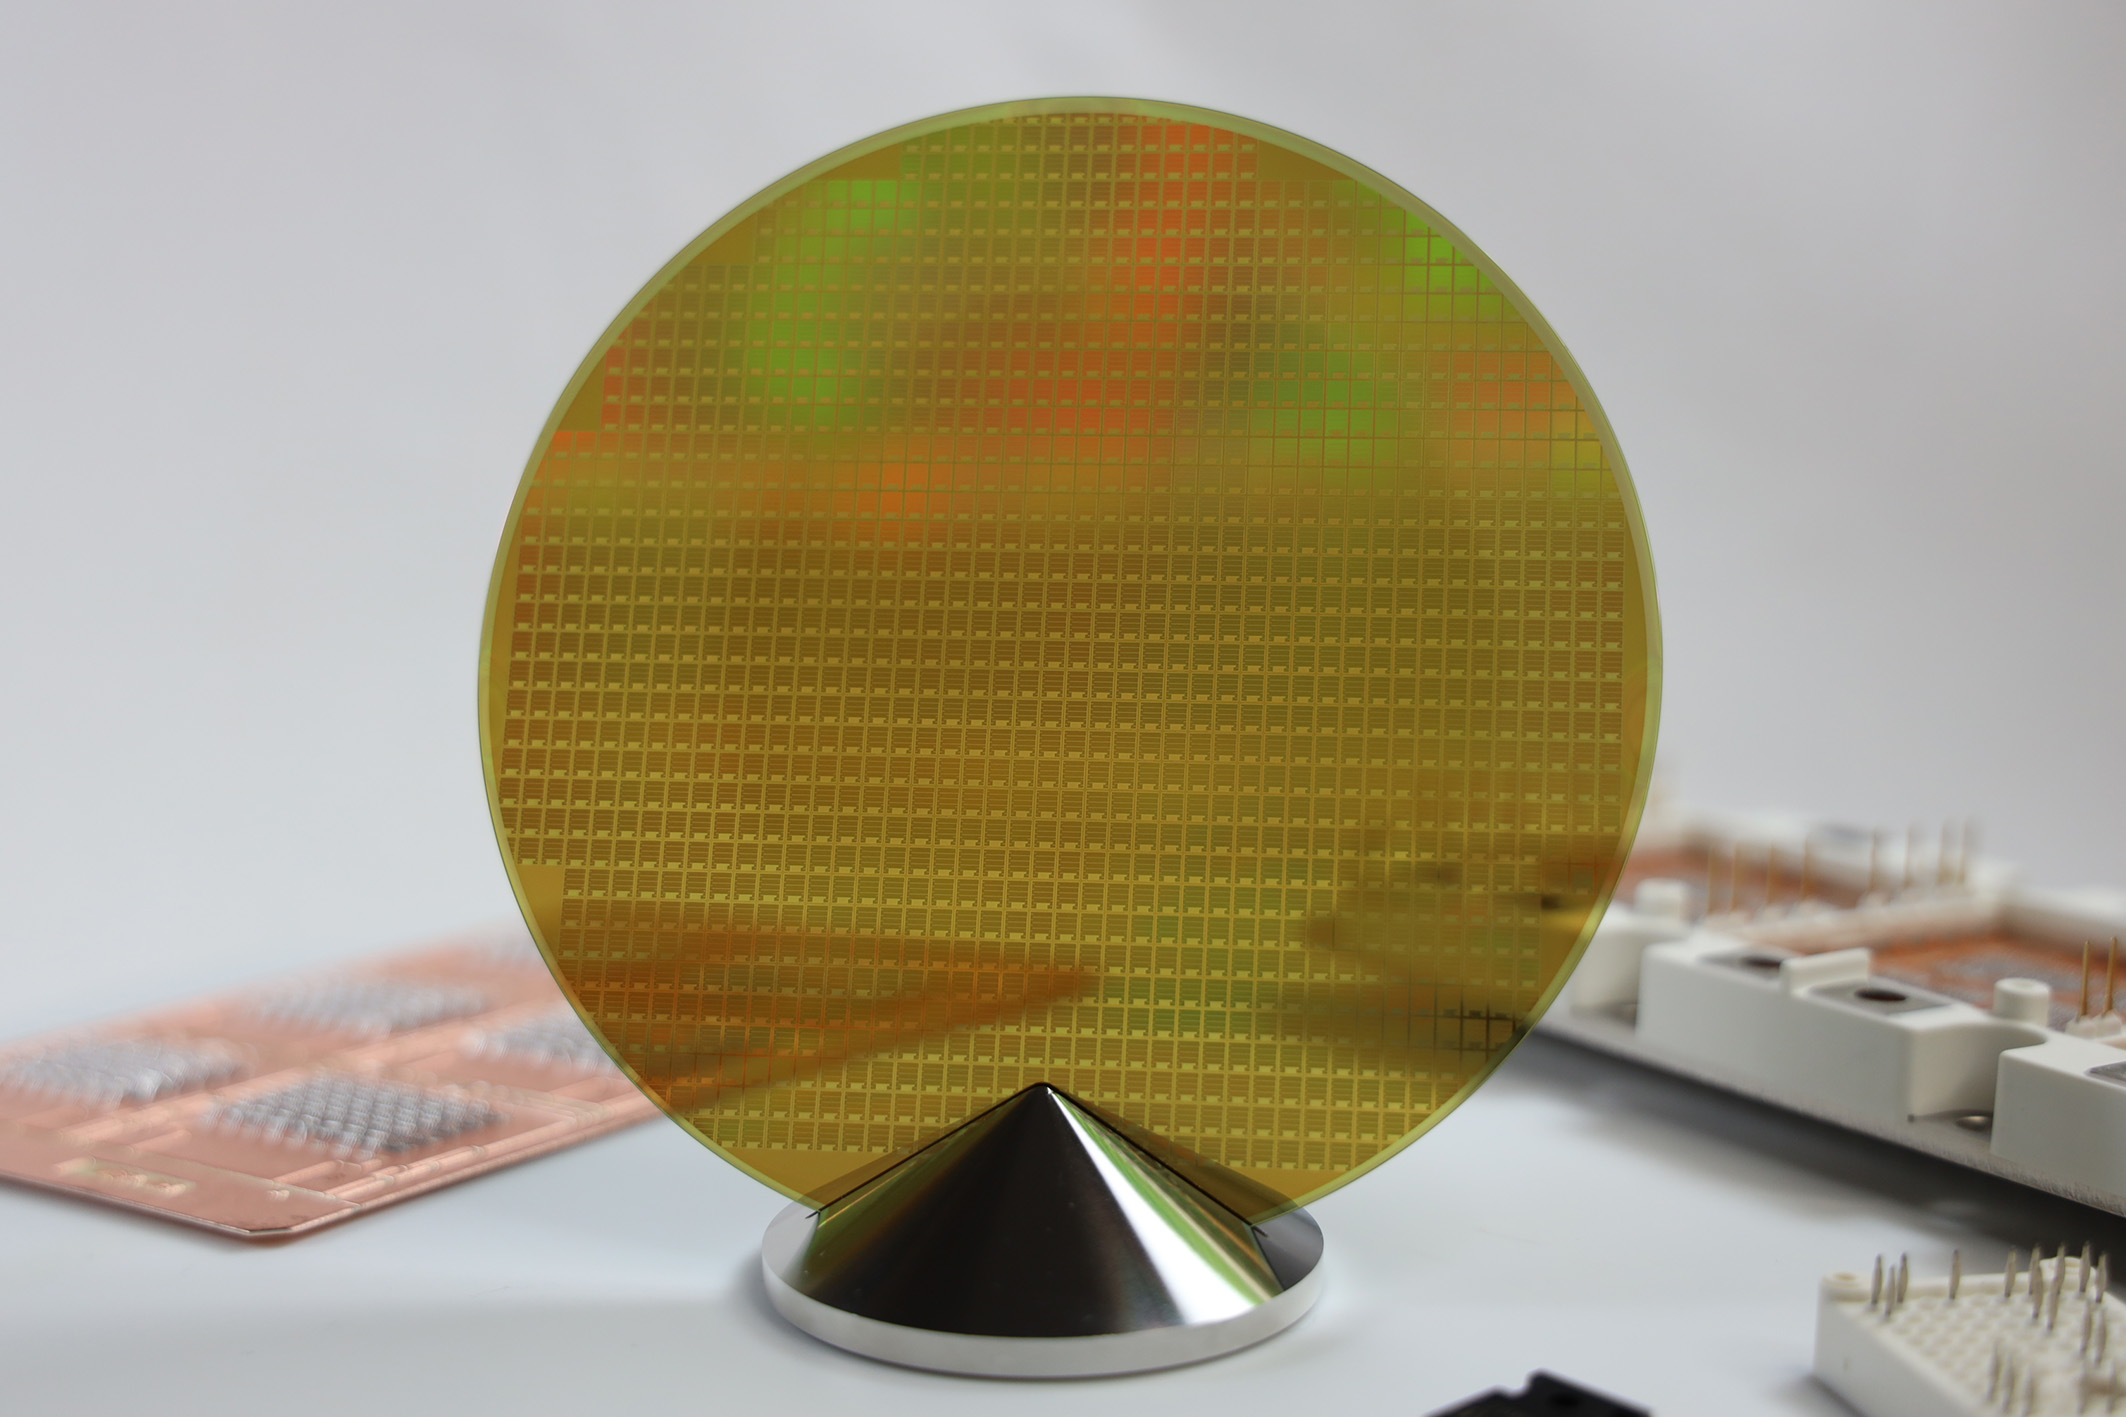
\includegraphics[width=0.9\textwidth]{bilder/SiC-Wafer-Infineon.jpg}
    \caption{Fertiger Silizium-Wafer mit Chips}
    \label{fig:Silizium-Wafer}
\end{figure}

Silizium ist das am häufigsten verwendete Material in der Halbleiterindustrie, weil es viele praktische Vorteile bietet. Es hat die perfekte Balance für den Einsatz in verschiedenen elektronischen Anwendungen und funktioniert gut bei normalen Betriebstemperaturen. Silizium bildet ein stabiles und zuverlässiges Isoliermaterial, das in Schaltkreisen vielseitig eingesetzt werden kann. Es leitet Wärme effizient ab, was wichtig ist, um eine Überhitzung zu vermeiden, besonders bei kleinen und leistungsstarken Chips. Außerdem lässt sich Silizium einfach in großen, reinen Kristallen herstellen, die für eine gleichmäßige Leistung in der Chipproduktion entscheidend sind.

Die Fertigung beginnt mit einem Rohwafer, auf dem im \gls{FEOL} alle Dotierungen erfolgen. Im darauf folgenden \gls{BEOL} werden abwechselnd isolierende und metallische Schichten aufgetragen und strukturiert, wodurch Leiterbahnen und Durchkontaktierungen entstehen. Die Strukturen moderner Chips sind dabei im Nano- bis Mikrometerbereich angesiedelt.

Am Ende des Fertigungsprozesses werden die integrierten Schaltkreise (\gls{IC}), die in parallelen Reihen und Spalten auf der Oberfläche des Wafers angeordnet sind, die in Abbildung \ref{fig:Silizium-Wafer} gut erkennbar sind, durch senkrecht verlaufende Schnitte voneinander getrennt. Durch diesen Schritt entstehen kleine, rechteckige, dünne Plättchen, die als Chips bekannt sind. Die Wafer, die aus den gezüchteten Kristallstäben mit Innenlochsägen ausgeschnitten werden, sind kreisrunde Scheiben und weisen typischerweise Dicken von knapp unter 1 mm auf. Die Durchmesser moderner Wafer liegen heute bei 200 bis 450 mm. Fortschrittliche Technologien wie die der Infineon Technologies AG ermöglichen jedoch bereits die Fertigung und Verarbeitung ultradünner Silizium-Wafer mit einer Dicke von nur 20 Mikrometern \cite{infineon2024dünnsterWafer}.

Mit zunehmender Miniaturisierung der Halbleiterprozesse steigen die Herstellungskosten, da die Technologie komplexer wird. Jedoch sinkt durch die Verkleinerung der benötigte Platz pro Funktionseinheit auf dem Chip, was die höheren Prozesskosten kompensieren kann. Dadurch führt jede neue Chip-Generation dazu, dass mehr Leistung für den gleichen Preis erzielt wird, also eine höhere Funktionalität pro investiertem Geld \cite{lienig2023halbleitertechnologie}.